\section{引言}

基准评测看起来很简单：我们在一组题目上运行模型并取平均。所得分数主要有两种用途：在排行榜上比较模型~\citep{alzahrani2024benchmarks,wang2018glue,liang2022holistic,myrzakhan2024open}，以及在训练过程中监测进展~\citep{liu2025prorl,hu2025open,he2025skywork,bercovich2025llama,luo2025deepscaler}。但这种简单性掩盖了一个基本问题：结论不仅取决于模型表现如何，也取决于基准题目如何分布~\cite{siska2024examining,zhang2026rankllm}。


首先考虑图~\ref{fig:teaser}(a) 中的排行榜设定，我们希望比较两个模型。假设它们在简单题上表现相近，但在难题上差异很大。若基准把大部分权重放在简单题上，而我们关心的难度分布把更多权重放在更难的题目上，则同对模型的两次评测可能得出不同结论：基准可能表明两个模型几乎打平，但在期望的难度分布下它们明显分开。再考虑图~\ref{fig:teaser}(b) 中的训练设定，我们希望追踪模型是否在改进。假设模型在某个局部难度区间上有\textit{显著}提升。若基准在该区域几乎没有或完全没有题目，基准分数可能几乎不变，尽管模型已经取得了真实进展。

这两个失效情形表明，基准结论关键取决于题目如何分布。为系统地研究这一结构，我们把基准题目排列在一条\textbf{难度}轴上，它提供了从较易到较难问题的自然递进。关键的概念步骤是用难度来定义基准自身的分布结构。这一观点将基准从一组测试题目，重构为难度上的一个\textbf{经验测度}，每道题在其难度水平上贡献相等的评测质量。


这种测度论形式化之所以有用，是因为它把上述两种失效情形转化为关于基准所诱导难度测度的精确、可分析问题。第一个是\textbf{测度失配}问题：基准分配质量的方式可能不同于代表预期评测目标的目标难度分布，因此基准结论可以不同于目标难度分布下的结论。第二个是\textbf{覆盖缺口}问题。由于基准是仅支撑在有限个难度点上的经验测度，可能存在几乎没有或完全没有基准质量的难度区间。集中在这样一个区间内的显著性能增益，因此可能几乎不改变、甚至完全不改变基准分数。据我们所知，这是首次将测度失配与覆盖缺口识别并形式化为基准评测的两种基本失效模式的工作。

这两个问题自然引出两个简单的诊断指标：基准测度与目标难度分布之间的 Wasserstein 距离~\cite{villani2009optimal}，以及相邻基准难度点之间的最大间隔。我们给出理论结果，表明这些量直接刻画分布失配以及局部改进的可检测性。在实验上，我们分析了涵盖 \textbf{7} 个领域的 \textbf{25} 个常用基准。我们用项目反应理论（Item Response Theory, IRT）估计题目难度并计算所提出的指标。结果表明，这两个问题在各类基准中普遍存在。

\textbf{我们的主要贡献概括如下：}
\vspace{0.2cm}
\begin{itemize}[wide, labelwidth=!, noitemsep, labelindent=0pt,topsep=-\parskip]
    \item 我们提出一种基于测度的基准评测新视角，将基准表示为难度上的经验测度。该视角形式化了测度失配与覆盖缺口，引出两个诊断指标，并给出严格的理论保证。

    \item 我们在涵盖 \textbf{7} 个领域的 \textbf{25} 个基准上开展实证研究，表明难度分布失配与大覆盖缺口在当前基准中广泛存在。

    \item 我们提出 \textsc{BenchFill}，一种面向目标难度的缺口填补算法。每个基准仅插入三道题，\textsc{BenchFill} 就将前三大难度间隔之和降低 $21.09\%$--$38.88\%$。
\end{itemize}

\begin{figure}[t]
    \centering
    \resizebox{\textwidth}{!}{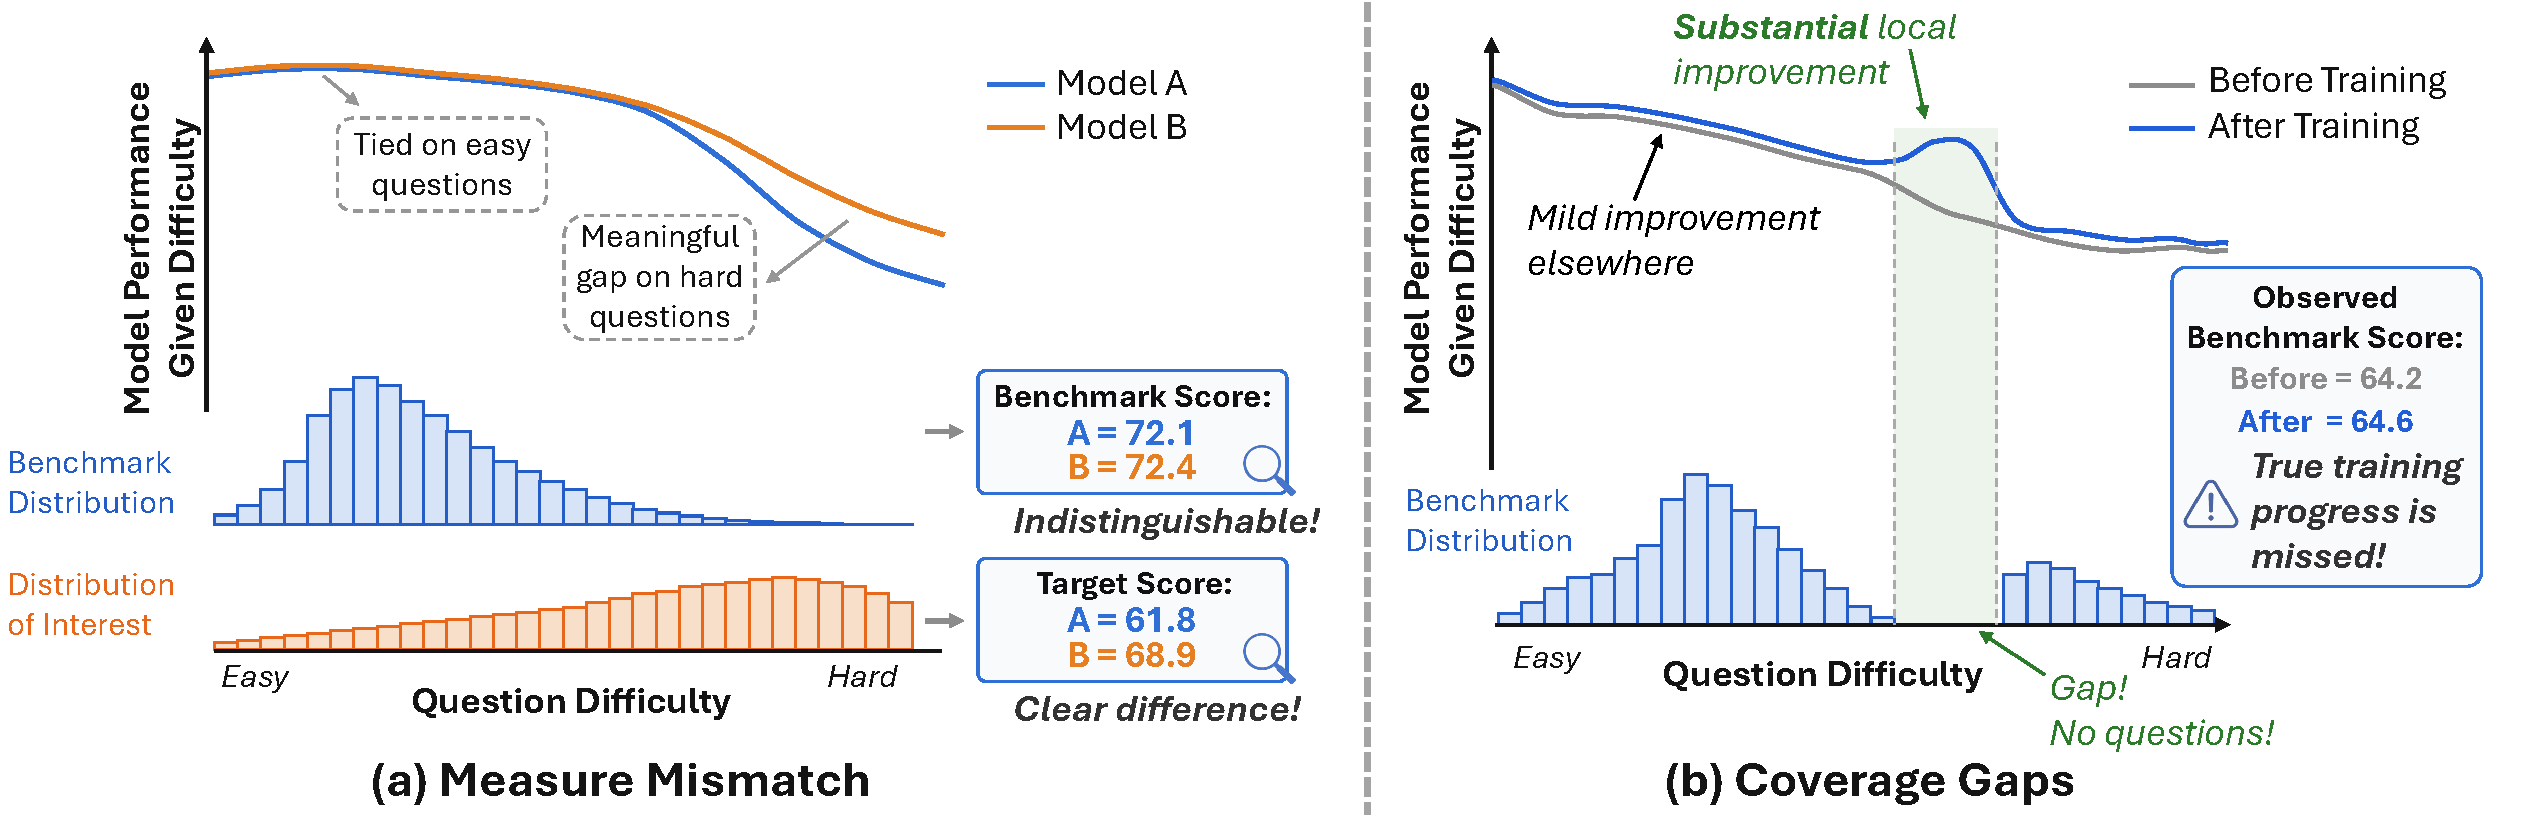
\includegraphics{Fig/teaser.pdf}}
      \vspace{-4mm}
    \caption{\textbf{两种基准失效情形。} 两幅图中的曲线均表示真实模型的\textit{条件}性能，即\textit{作为题目难度的函数}。
    (a) \textbf{测度失配。}
    基准强调简单题，而模型在简单题上表现相近；我们关心的难度分布则把更多权重放在更难的题目上，模型在这些题目上差异很大。
    由于基准与目标分布对难度轴的加权不同，它们对同一对模型给出不同结论。
    % As a result, the benchmark suggests a near tie, whereas the target evaluation shows a clear separation.
    (b) \textbf{覆盖缺口。} 模型实际上在某个局部难度区域上有\textit{显著}提升。由于基准在该区域没有题目，这一提升没有反映在观测到的基准分数中，导致有意义的训练进展被遗漏。}
    \label{fig:teaser}
  \vspace{-6mm}
\end{figure}
